\begin{frame}{Modelo relacional}
    \centering
    \Huge \textcolor{blue3}{Estructura de datos}

    \note{@NOTE cu\'al es el modelo matem\'atico de datos para el modelo relacional}
\end{frame}

\begin{frame}{¿C\'omo describir una tabla?}
    \begin{LARGE}
        
        ¿Qu\'e conceptos matem\'aticos pudiesen modelar una tabla?
    \end{LARGE}
    


    \begin{center}
        JUGADOR
        \vspace{2mm}

        \begin{tabular}{|c|c|c|c|c|}
            \hline
            \underline{\#J} & Nombre & Nivel& Trofeos & TrofeosMax\\
            \hline
            1 & Juan & 13 & 7500 & 7560\\
            \hline
            2 & Pedro &  11 & 7000 & 7200 \\
            \hline
            3 & Mar\'ia & 12  & 7050 & 7400\\
            \hline
            $\vdots$ & $\vdots$ & $\vdots$ & $\vdots$ & $\vdots$\\
            \hline
            
        \end{tabular}
    \end{center}
   
\end{frame}

\begin{frame}{¿Nos servir\'a alguna estructura matem\'atica que ya conocemos?}
    \centering
    \begin{LARGE}
        
        ¿Podemos utilizar una matriz?
    \end{LARGE}
    
    \vspace{5mm}

    \[
  A_{m\times n} =
  \left[ {\begin{array}{cccc}
    a_{11} & a_{12} & \cdots & a_{1n}\\
    a_{21} & a_{22} & \cdots & a_{2n}\\
    \vdots & \vdots & \ddots & \vdots\\
    a_{m1} & a_{m2} & \cdots & a_{mn}\\
  \end{array} } \right]
\]

\vspace{5mm}

\onslide<2>{
\centering
    \begin{LARGE}
       \textcolor{red}{No. Las matrices se definen sobre un \'unico dominio}
    \end{LARGE}
}



\end{frame}

\begin{frame}{¿Nos servir\'a alguna estructura matem\'atica que ya conocemos?}

    \begin{block}{Dominio}
        Conjunto de valores que puede tomar un atributo.
    \end{block}

    \onslide<2>{
    \begin{block}{Relaci\'on (Teor\'ia de conjuntos)}
       La relaci\'on $n$-aria sobre los dominios $D_1,D_2,...,D_n$
       es el conjunto de tuplas ordenadas $(a_1,a_2,...,a_n)$ pertenecientes
       al producto cartesiano $D_1 \times D_2 \times ... \times D_n$, donde
       $a_i \in D_i$, para cada $i\in{1,...,n}$, cuya condici\'on $R(a_1,a_2,...,a_n)$ se satisface.

       $$
        R = \{(a_1,a_2,...,a_n) \in D_1 \times D_2 \times ... \times D_n \,|\, R(a_1,a_2,...,a_n)\}
       $$

    \end{block}
    }
\end{frame}

\begin{frame}{¿Se podr\'ia mejorar?}
   \centering
    \begin{tikzpicture}
        \node {
            \begin{minipage}{0.50\textwidth}
                
                \[ \text{JUGADOR} = \left \{ \begin{array}{c}
                
                    <1,\text{Juan},13,7500,7560>, \\
                    <2,\text{Pedro},11,7000,7200>, \\
                    <3,\text{Mar\'ia},12,7050,7400>,\\
                    \vdots
                \end{array} \right \} \] 
            \end{minipage}    
        };

        \onslide<2>{
        \draw[->, color=red] (2,2) -- (1.3,1);
        \draw[->, color=red] (2,2) -- (0,1);
        \node at (2, 2.3) {\textcolor{red}{¿C\'omo el usuario distingue entre el identificador y el nivel?}};
        }

        \onslide<3>{
        \draw[->,color=red] (0.5,2) -- (0.5,1);
        \node at (2, 2.3) {\textcolor{red}{El usuario debe recordar que el nombre es el segundo elemento}};
        }
    \end{tikzpicture}

    \begin{alertblock}<2->{Problemas}
        \begin{itemize}
            \item<2-> No es autodescriptiva
            \item<3-> El orden de los datos importa
        \end{itemize}
    \end{alertblock}

       
   

    
    
\end{frame}



\begin{frame}[fragile]{¿C\'omo usar relaciones para almacenar registros?}
    \begin{block}{Relaci\'on (Bases de datos)}
        Una relaci\'on $R$ definida sobre un conjunto de dominios
        $D_1, D_2, ..., D_n$, no necesariamente distintos, se compone de:
        \begin{itemize}
            \item La \textbf{cabecera}, formada por un conjunto finito de pares atributo-dominio
            $$
                \{(A_1:D_1), (A_2:D_2), ..., (A_n:D_n)\}
            $$
            tal que el atributo $A_j$ corresponde al y s\'olo al dominio $D_j$ para todo\\ $j=1,2,...,n$. 
        \end{itemize}
        \vspace{3mm}

        \onslide<2>{
        \begin{center}
            \small{Cabecera para la relaci\'on Jugador}\\[2mm]

            $
            \{ (\text{\#J} : \mathbb{N}), (\text{Nombre} : \mathbb{S}),
            (\text{Nivel} : \mathbb{N}),  (\text{Trofeos} : \mathbb{N}),  (\text{TrofeosMax} : \mathbb{N}) \}
            $
            \\[1mm]
            $
                \mathbb{S} = \{\text{Conjunto de todas las cadenas de longitud} \leq 20\}
            $

            
        \end{center}
        }

      

    

\end{block}


    \note<2>{@NOTE recalcar que 2 atributos son iguales si tienen dominios =s tambie'n}
\end{frame}

\begin{frame}{¿C\'omo usar relaciones para almacenar registros?}
    \begin{block}{Relaci\'on (Bases de datos)}
        Una relaci\'on $R$ definida sobre un conjunto de dominios
        $D_1, D_2, ..., D_n$, no necesariamente distintos, se compone de:
        \begin{itemize}
            \item El \textbf{cuerpo}, est\'a formado por un
            conjunto finito de tuplas, el cual var\'ia en el tiempo.
            Cada tupla, a su vez, est\'a formada por un conjunto de pares
            atributo-valor.
            $$
                \{(A_1:V_{i1}),(A_2:V_{i2}),...,(A_n:V_{in})\}, \ (i=1,2,...,m)
            $$
            tal que $m$ es la cantidad de tuplas en el conjunto y 
            $V_{ij} \in D_j$ para todo par $(A_j:V_{ij})$ con $j=1,2,...,n$
            
        \end{itemize}
        \vspace{3mm}

        \onslide<2>{
            \begin{center}
                \small{Ejemplo de tupla para la relaci\'on Jugador}\\[2mm]

                $
                \{ (\text{\#J} : 1), (\text{Nombre} : \text{Juan}),
                (\text{Nivel} : 13),  (\text{Trofeos} : 7500),  (\text{TrofeosMax} : 7560) \}
                $
            \end{center}
        }
    \end{block}
\end{frame}


\begin{frame}{Identificando registros}
    \begin{block}{Llave candidata}
        Un conjunto de uno o m\'as atributos $K = \{A_1,A_2,...,A_n\}$ es una llave candidata
        de la relaci\'on $R$ si cumple las siguientes propiedades:
        \begin{enumerate}
            \item \textbf{Unicidad}: En cualquier momento dado, no existen dos tuplas
            distintas de $R$ con los mismos valores para $A_1,A_2,...,A_n$.
            \item \textbf{Minimalidad}: Ning\'un subconjunto propio de $K$ tiene la
            propiedad de unicidad.
        \end{enumerate}
    \end{block}

    \begin{block}{Llave primaria}
        Es una de las llaves candidatas que se selecciona
        como llave de la relaci\'on.
    \end{block}
    
\end{frame}

\begin{frame}{Representando relaciones}
    \centering
    \resizebox{!}{3cm}{
    \begin{tikzpicture}[node distance=6em]
        \tikzstyle{every entity} = [minimum width=2cm, minimum height=1.2cm]
        \node[entity] (jugador) {JUGADOR}
            [sibling distance=3cm]
            child {node[attribute] [above right of=jugador] {\tiny TROFEOS MAX}}
            child {node[attribute] [above of=jugador] {\tiny TROFEOS}}
            child {node[attribute] [above left of=jugador] {\tiny NOMBRE}}
            child {node[attribute] [left of=jugador] {\underline{\tiny \#J}}}
            child {node[attribute] [right of=jugador] {\tiny NIVEL}}
            ;
       
        \node[entity] (carta) at (8,0) {CARTA}
        [sibling distance=3cm]
        child {node[attribute] [right of=carta] {\underline{\tiny \#C}}}
        child {node[attribute] [above of=carta] {\tiny NOMBRE}}
        child {node[attribute] [above left of=carta] {\tiny CALIDAD}}
        child {node[attribute] [above right of=carta] {\tiny DESC}}
        child {node[attribute] [left of=carta] {\tiny COSTO}};

    \end{tikzpicture}
    }\\[2mm]

    \begin{block}{}
        
        \hspace{20mm}Jugador(\underline{\#J}, Nombre, Nivel, Trofeos, TrofeosMax)\\
        \hspace{20mm}Carta(\underline{\#C}, Nombre, Calidad, Desc, Costo)\\
        
    \end{block}

    \note{@NOTE la llave primaria se subraya en la relaci\'on. Recuerden q puede ser compuesta}
\end{frame}


\begin{frame}{Relaciones para almacenar interrelaciones}
    \begin{block}{Llave for\'anea}
        Un conjunto de uno o m\'as atributos $F = \{A_1, A_2,...,A_n\}$ de una relaci\'on $R$, correspondientes
        a los dominios $D_1, D_2,...,D_n$ respectivamente, es una llave for\'anea referente a la relaci\'on $R'$ si:
        \begin{enumerate}
            \item La llave primaria de $R'$ es un conjunto de atributos $P = \{B_1,B_2,...,B_n\}$ correspondientes
            a los dominios $D_1,D_2,...,D_n$ respectivamente.
            \item Existe un acuerdo de correspondencia entre los atributos $A_i$ y $B_i$ para todo $i = 1,2,...,n$
           
        \end{enumerate}

        Una tupla $t \in R$ referencia a una tupla $t' \in R'$ si el valor de $A_i$ en la tupla $t$ es igual al valor
        de $B_i$ en la tupla $t'$ para todo $i=1,2,...,n$.
    \end{block}

\end{frame}

\begin{frame}{Interrelacionando registros: ejemplo}
    \begin{columns}[T]
        \begin{column}{0.48\linewidth}
            \begin{center}
                \vspace{10mm}
                \resizebox{\linewidth}{!}{
                \begin{tikzpicture}[node distance=6em]
                    \tikzstyle{every entity} = [minimum width=2cm, minimum height=1.2cm]
                    \node[entity] (jugador) {JUGADOR}
                        [sibling distance=3cm]
                        child {node[attribute] [above right of=jugador] {\tiny TROFEOS MAX}}
                        child {node[attribute] [above of=jugador] {\tiny TROFEOS}}
                        child {node[attribute] [above left of=jugador] {\tiny NOMBRE}}
                        child {node[attribute] [left of=jugador] {\underline{\tiny \#J}}}
                        child {node[attribute] [below left of=jugador] {\tiny NIVEL}}
                        ;
                   
                    \node[entity] (carta) at (8,0) {CARTA}
                    [sibling distance=3cm]
                    child {node[attribute] [right of=carta] {\underline{\tiny \#C}}}
                    child {node[attribute] [above of=carta] {\tiny NOMBRE}}
                    child {node[attribute] [above left of=carta] {\tiny CALIDAD}}
                    child {node[attribute] [above right of=carta] {\tiny DESC}}
                    child {node[attribute] [below right of=carta] {\tiny COSTO}};

                    \node[relationship,aspect=2] (pertenecer) at (4,0) {COLECCIONAR}
                    edge(jugador) edge(carta);

                    \node at (1.3, 0.2) {$\ast$};
                    \node at (6.7, 0.2) {$\ast$};
                \end{tikzpicture}
                }
            \end{center}
        \end{column}

        \begin{column}{0.48\linewidth}
            \resizebox{\linewidth}{!}{
                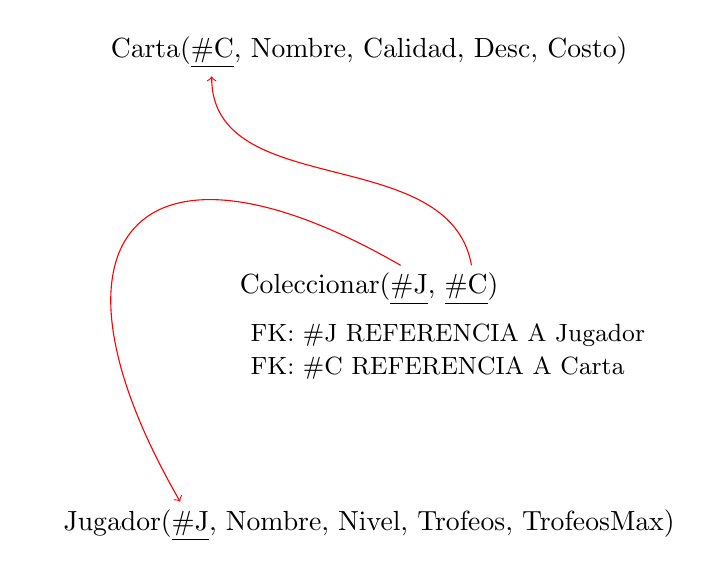
\begin{tikzpicture}
                    \node {Jugador(\underline{\#J}, Nombre, Nivel, Trofeos, TrofeosMax)};
                    \node at (0,6) {Carta(\underline{\#C}, Nombre, Calidad, Desc, Costo)};
                    \node at (0,3) { Coleccionar(\underline{\#J}, \underline{\#C})};
                    \node[align=left] at (1,2.2) {\small FK: \#J REFERENCIA A Jugador\\
                                                    \small FK: \#C REFERENCIA A Carta };

                    \path[->, color=red] (0.4,3.3) edge [out=150,in=120, looseness=2.4] (-2.4,0.3);
                    \path[->, color=red] (1.3,3.3) edge [out=100,in=270] (-2,5.7);
                    
                \end{tikzpicture}
            }
        \end{column}
        
    \end{columns}
    
    \note{@NOTE MUCHOS-MUCHOS}
\end{frame}


\begin{frame}{Interrelacionando registros: ejemplo}
    \begin{columns}[T]
        \begin{column}{0.48\linewidth}
            \centering
            \resizebox{\linewidth}{!}{
                \begin{tikzpicture}[node distance=6em]
                    \tikzstyle{every entity} = [minimum width=2cm, minimum height=1.2cm]
                    \node[entity] (jugador) {JUGADOR}
                        [sibling distance=3cm]
                        child {node[attribute] [above right of=jugador] {\tiny TROFEOS MAX}}
                        child {node[attribute] [above of=jugador] {\tiny TROFEOS}}
                        child {node[attribute] [above left of=jugador] {\tiny NOMBRE}}
                        child {node[attribute] [left of=jugador] {\underline{\tiny \#J}}}
                        child {node[attribute] [below left of=jugador] {NIVEL}}
                        ;
                  
                    \node[entity] (clan) at (8,0) {CLAN}
                    [sibling distance=3cm]
                    child {node[attribute] [right of=clan] {\underline{\tiny \#Cl}}}
                    child {node[attribute] [above of=clan] {\tiny REGI\'ON}}
                    child {node[attribute] [above left of=clan] {\tiny TIPO}}
                    child {node[attribute] [above right of=clan] {\tiny NOMBRE}}
                    child {node[attribute] [below right of=clan] {\tiny TROFEOS MIN}};

                    \node[relationship,aspect=2] (pertenecer) at (4,0) {SER\_L\'IDER}
                    edge(jugador) edge(clan);

                    \node at (1.5, 0.25) {$1,1$};
                    \node at (6.5, 0.25) {$0,1$};
                \end{tikzpicture}
            }
        \end{column}

        \begin{column}{0.48\linewidth}
            \resizebox{\linewidth}{!}{
                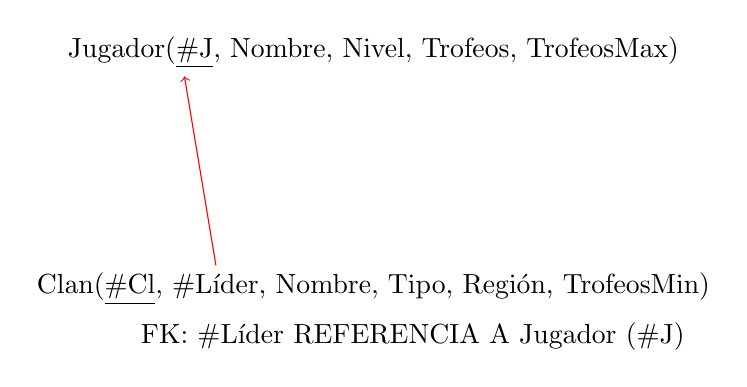
\begin{tikzpicture}
                    \node at (0,3){Jugador(\underline{\#J}, Nombre, Nivel, Trofeos, TrofeosMax)};
                    \node  {Clan(\underline{\#Cl}, \#L\'ider, Nombre, Tipo, Regi\'on, TrofeosMin)};
                    \node at (0.5,-0.6) {FK: \#L\'ider REFERENCIA A Jugador (\#J)};
                    \draw[->,color=red] (-2, 0.3) -- (-2.4,2.7);
                    
                \end{tikzpicture}
            }
        \end{column}
    \end{columns}
\end{frame}

\begin{frame}{Identificando relaciones}
    \begin{block}{Esquema de una relaci\'on}
        El esquema de una relaci\'on es una especificaci\'on de su estructura, la cual
        es independiente de las tuplas
        que contiene el cuerpo. El esquema se compone de: \begin{itemize}
            \item El nombre de la relaci\'on
            \item La cabecera
            \item La llave primaria
            \item Las llaves for\'aneas
        \end{itemize}
        En una misma base de datos una relaci\'on se identifica un\'ivocamente por su nombre.
    \end{block}

    \onslide<2>{
    \begin{block}{Instancia de una relaci\'on}
        Se refiere al conjunto de tuplas que constituye el cuerpo de la relaci\'on en un
        momento espec\'ifico del tiempo.
    \end{block}
    }
\end{frame}

\begin{frame}{Identificando relaciones: ejemplo}

    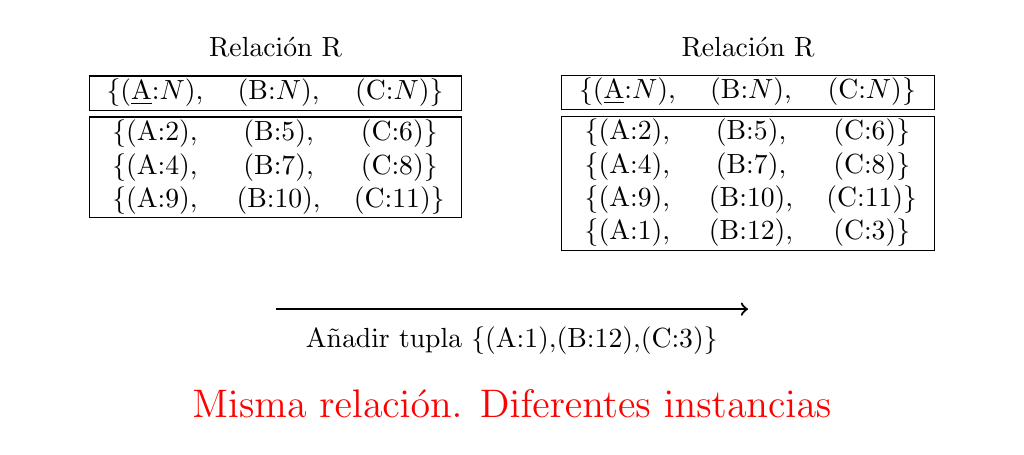
\begin{tikzpicture}
        \node at (0,0) {
            \begin{minipage}{0.50\textwidth}
                \centering
                Relaci\'on R\\[2mm]
                \begin{tabular}{|ccc|}
                    \hline
                    \{(\underline{A}:$\mathbb{N}$), & (B:$\mathbb{N}$), & (C:$\mathbb{N}$)\}\\
                    \hline
                    \hline
                    \{(A:2), & (B:5), & (C:6)\}\\
                    \{(A:4), & (B:7), & (C:8)\}\\
                    \{(A:9), & (B:10), & (C:11)\}\\
                    \hline
                \end{tabular}
            \end{minipage}    
        };
        \node at (6,-0.2) {
            \begin{minipage}{0.50\textwidth}
                \centering
                Relaci\'on R\\[2mm]
                \begin{tabular}{|ccc|}
                    \hline
                    \{(\underline{A}:$\mathbb{N}$), & (B:$\mathbb{N}$), & (C:$\mathbb{N}$)\}\\
                    \hline
                    \hline
                    \{(A:2), & (B:5), & (C:6)\}\\
                    \{(A:4), & (B:7), & (C:8)\}\\
                    \{(A:9), & (B:10), & (C:11)\}\\
                    \{(A:1), & (B:12), & (C:3)\}\\
                    \hline
                \end{tabular}
            \end{minipage}    
        };

        \draw[->,thick] (0,-2.3) -- (6,-2.3);

        \node at (3,-2.7) {A\~nadir tupla \{(A:1),(B:12),(C:3)\}};

        \node at (3,-3.5) {\Large \textcolor{red}{Misma relaci\'on. Diferentes instancias}};

    \end{tikzpicture}
\end{frame}


\begin{frame}{Modelo relacional}
    \vspace{5mm}
    \begin{overlayarea}{\linewidth}{\textheight}
        \begin{block}{Estructura de datos}
           Relaci\'on
        \end{block}
    \end{overlayarea}
\end{frame}


% \begin{frame}{Definiendo la abstracci\'on}

%     \hspace{8mm}\texttt{\kword{namespace} \tword{RelationalModel};}\\
%     \hspace{8mm}\texttt{\kword{using} \tword{RelationalTuple} = \tword{IDictionary}<\kword{string}, \kword{object}>;}\\[3mm]

%     \hspace{8mm}\texttt{\kword{public abstract class} \tword{Relation} \{ }\\[3mm]

%     \hspace{16mm}\texttt{\kword{public} \tword{IDictionary}<\kword{string}, \tword{Type}> Header \{\kword{get}; \kword{set};\}}\\
%     \hspace{16mm}\texttt{\kword{public} \tword{ISet}<\tword{RelationalTuple}> Body \{\kword{get}; \kword{set};\}}\\[3mm]

    
%     \hspace{16mm}\texttt{\kword{public} \tword{ISet}<\kword{string}> PrimaryKey \{\kword{get}; \kword{set};\}}\\
%     \hspace{16mm}\texttt{\kword{public} \tword{IDictionary}<\tword{Relation}, \tword{IDictionary}<\kword{string}, \kword{string}>> ForeignKeys \{\kword{get}; \kword{set};\}}\\
%     \hspace{8mm}\texttt{\}}
% \end{frame}






